% Chapte 9
\chapter{Advertisement enhancement} % Main chapter title

\label{Chapter9} % For referencing the chapter elsewhere, use \ref{Chapter1} 
\newpage






\section{Introduction}




Advertisement enhancement is another follow-up study of the previous experiment in which the body interaction was found to be the most attractive and engaging advertisement compared to the other two techniques (Non-interactive and mobile Interactive), 






\section{Advertisement enhanced version}

The advertisement interface was exactly the same, but the only change was brought in it was the integration of multiple Kinect cameras to cover the sides of the screen, a person passing from the side could see his self at the side of the screen and when moving to the middle of the screen the camera could smoothly transition the person from side camera to the center camera by having the same silhouette color, physically the cameras are positioned side-by-side therefor there is a small gap for each camera range, which is also not perceivable by passers-by. Refere to chapter 7 for more technical details.


\begin{figure}[H]
    \centering
    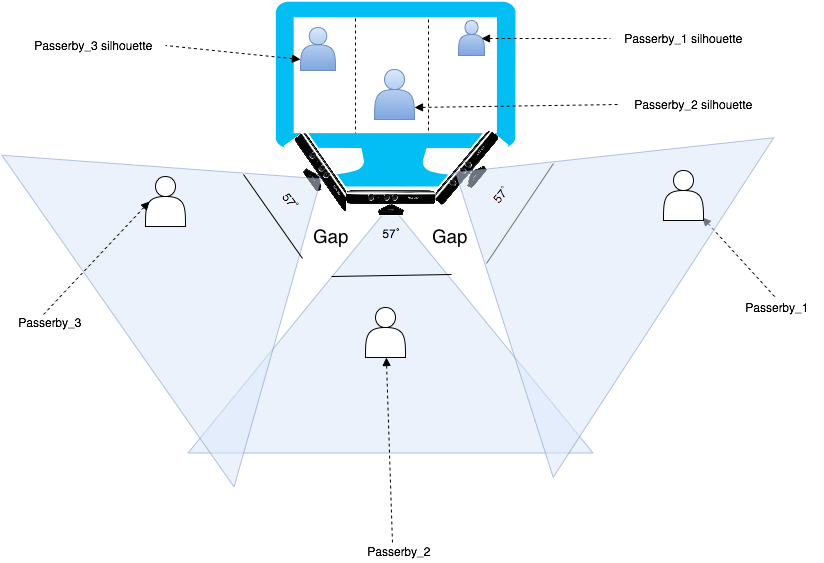
\includegraphics[width=110mm,height=70mm]{Figures/9/Kinect_Extended}
    \caption{Advertisement extended version using three Kinect cameras.}%
    \label{fig:KinectExtended}%
\end{figure}




\section{Research question}
This experiment was conducted to find out that what are the major effects when the coverage area is expanded in both right and left side of the screen.

\begin{enumerate}
\item Would the attention level change?
\item Would the number of engaged passers-by increase?
\item Would the average engagement time rise?
\item Would there be any changes in number of Honeypot and landing effect?
\item What would be other passer-by behavior to the screen?
\end{enumerate}



\section{Design study}

\subsection{Location}
The same location that the last experiment was conducted was chosen again, it was in Weimar tourist information center, It was positioned in the same pathway of passers-by. 


\subsection{Duration}
This experiment was conducted only with advertisement’s extended version for three continues days; the days were the crowded days of the week (Friday, Saturday, Sunday), 

\subsection{Participants}
The participants were from Tourist information center; they were not informed that there is an interactive screen. Most of the participants were of old age, and the rest were middle aged and young aged participants. 

\subsection{Data gathering}
The bellow types of data were gathered during three days.


\begin{enumerate}
\item \textbf{On-Site Observation} \\
Observation periods were selected the same as the previous study, from 10:00 – 12:00 and the second was from 14:00 – 16:00, During these two time slots the bellow observations were made.

\begin{enumerate}
\item \textbf{Attention Level measurement} \\
Number of glances and number of ignores were counted by observing the passers-by from a fixed location, anyone who turned his/her face less than 3 seconds were counted as glance, see the full report of glances in Appendix \ref{AppendixE}.1

\item \textbf{Passerby behavior} \\
The behaviors of the passers-by were observed by direct observation in onsite and also from the Camera depth recorded frames. From the observation two important effects were taken in consideration (honeypot and landing effect).


\end{enumerate}

\item \textbf{Colored-image recording} \\
A 2D colored image was taken per second from each of three cameras, and meanwhile were joint together side-by-side and after the image recording was done, in lab another post processing script was applied to integrate a static background using Adobe Photoshop application. To match the data logs and the image frames each image name consisted time as (12.43.21.png).

\begin{figure}[H]
   \centering
    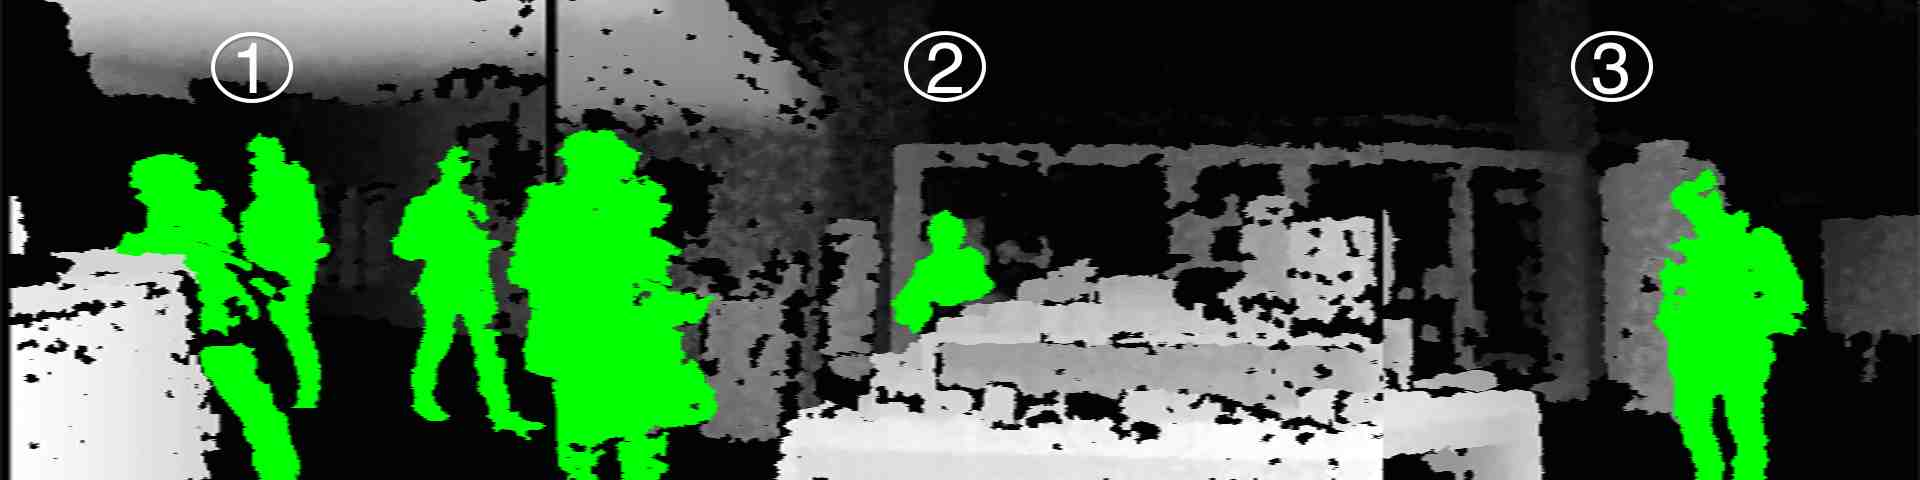
\includegraphics[width=\textwidth,height=50mm]{Figures/9/stacked_image}%
    \caption{Three kinect images stacked together, as can be seen that people' colored images rendered on the images (1,2 and 3) these images are stacked together so that the transition of one person be smooth from one camera to the other. }%
    \label{fig:threekinectimages}%
\end{figure}

\end{enumerate}


\section{Findings and results}



\subsection{Attention Level measurements}

\begin{figure}[H]
    \centering
    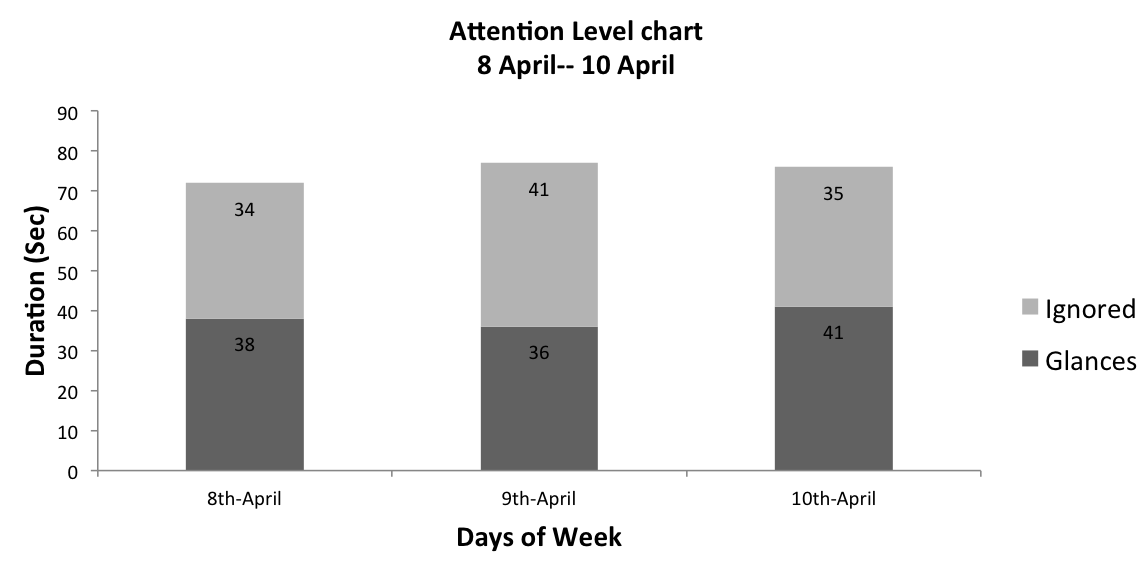
\includegraphics[width=110mm,height=55mm]{Figures/9/newbody_Inter_chart}%
    \caption{New body interactive attention level chart}%
    \label{fig:newbodyattentionlevelchart}%
\end{figure}



\begin{figure}[H]
    \centering
    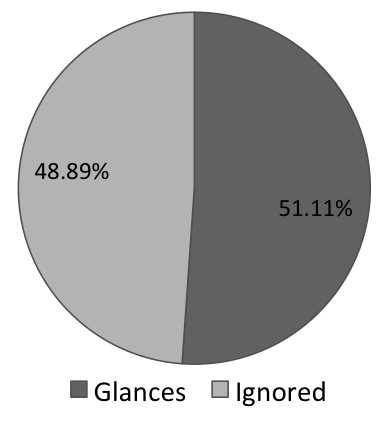
\includegraphics[width=110mm,height=55mm]{Figures/9/newbody_inter_percentage}
    \caption{Non-interactive Attention level percentage}%
    \label{fig:Nonattentionlevelpercentage}%
\end{figure}



\subsection{Engagement time}

\subsection{Passerby and engagement}



\begin{figure}[H]
    \centering
    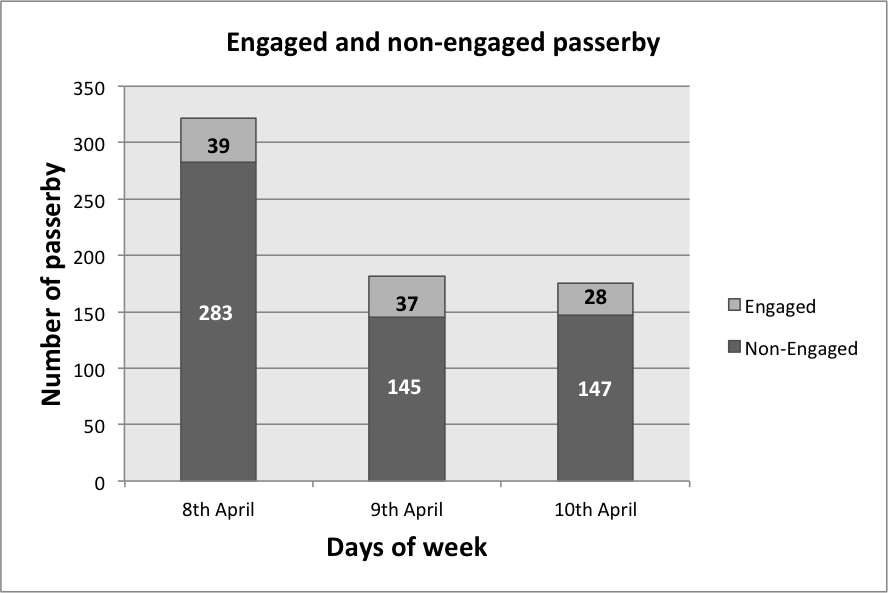
\includegraphics[width=110mm,height=60mm]{Figures/9/newbody_inter_engage_day}
    \caption{New body interaction Number of engaged passerby}%
    \label{fig:newbodyengagedandengagedby}%
\end{figure}

\begin{figure}[H]
    \centering
    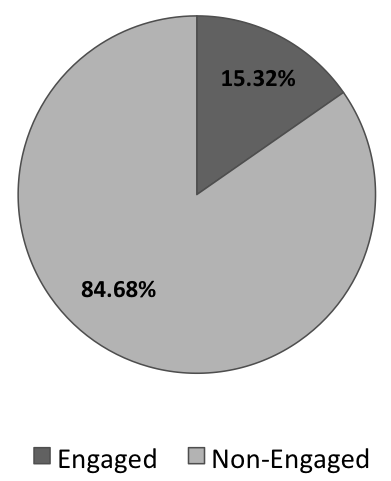
\includegraphics[width=110mm,height=60mm]{Figures/9/newbody_eng_percentage}
    \caption{New body Percentage of engaged and passerby}%
    \label{fig:newbodyengagedpasserbypercentage}%
\end{figure}




\subsection{Landing and Honeypot effects}

\begin{table}[H]
\caption{Landing and honeypot effects}
\label{tab:landingandhonypot}
\centering
\begin{tabular}{| l | c | c |}
\toprule
\tabhead{Days} & \tabhead{Landing effect} & \tabhead{Honeypot effect} \\
\midrule
\textbf{8th April}  & 3 &  3 \\
\textbf{9th April}  & 2 &  5 \\
\textbf{10th April}  & 1 &  2 \\
\bottomrule
\end{tabular}
\end{table}


\subsection{Note taking}

see Appendix Appendix \ref{AppendixE}.2

\subsection{Comparison with Body interaction}


\begin{enumerate}


\item Comparison of number of passerby
To be on safe side that the number of participants were statistically the same the bellow computation has be applied.
\begin{table}[H]
\caption{Number of people for three conditions}
\label{tab:newbodypasserbyofthreeweeks}
\centering
\begin{tabular}{| l | c | c | c |}
\toprule
\tabhead{Days} & \tabhead{Non-Interactive} & \tabhead{Body Interactive} & \tabhead{New-body Interactive} \\
\midrule
\textbf{Day 1}  & 212 & 259 &  322 \\
\midrule
\textbf{Day 2}  & 209 & 216 &  182 \\
\midrule
\textbf{Day 3}  & 208 & 122 &  175 \\
\midrule
\textbf{Total}  & 629 & 597 &  679 \\
\bottomrule
\end{tabular}
\end{table}


ANOVA test revealed that there is no significant different between the passers-by in each of the conditions (\emph{(F2,3)=0.1449, p >.05 (p=0.868)})



\item{Attention Level measurements}

\begin{table}[H]
\caption{Cross tabulation for each condition attention level }
\label{tab:newbodycrosstabulationweeks}
\centering
\begin{tabular}{| l | c | c | c |}
\toprule
\tabhead{Method} & \tabhead{Glanced (\%)} & \tabhead{Ignored} & \tabhead{Total } \\
\midrule
\textbf{Body Interactive}     	 & 96 (\%38.70)   &   152      &   248\\
\midrule
\textbf{New body Interactive }   & 108 (\%49.54)  &   110      &   218\\
\midrule
\textbf{Total }         		 & 204            &   262      &   466\\
\bottomrule
\end{tabular}
\end{table}

As can be seen the new body interactive advertisement has a higher percentage almost \%50 of the glances compared to the old body interactive advertisement.

To see if these are statistically significant different, the Chi-square test was applied on them.\\
${\chi}^2$\emph{(1, N=466)=5.5303, p < .05 (p=.01869)}





\item{Landing effects}


\begin{table}[H]
\caption{Cross tabulation for each condition Landing effect }
\label{tab:newbodylandingeffect}
\centering
\begin{tabular}{| l | c | c | c |}
\toprule
\tabhead{Method} & \tabhead{Non-Interactive} & \tabhead{Body Interactive} & \tabhead{New body Interactive } \\
\midrule
\textbf{Day 1}    & 2    &   2      &   1\\
\midrule
\textbf{Day 2 }   & 0    &   2      &   2\\
\midrule
\textbf{Day 3}    & 1    &   3      &   3\\
\bottomrule
\end{tabular}
\end{table}

ANOVA states that there is no significant different for these three days for all of the conditions.\\
(\emph{(F2,3)=1.857, p >.05 (p=0.236)})


\item{Honeypot effects}


\begin{table}[H]
\caption{Cross tabulation for each condition Honeypot effect }
\label{tab:newbodyhoneypoteffect}
\centering
\begin{tabular}{| l | c | c | c |}
\toprule
\tabhead{Method} & \tabhead{Non-Interactive} & \tabhead{Body Interactive} & \tabhead{New body Interactive } \\
\midrule
\textbf{Day 1}    & 2    &   2      &   3\\
\midrule
\textbf{Day 2 }   & 2    &   5      &   5\\
\midrule
\textbf{Day 3}    & 1    &   3      &   2\\
\bottomrule
\end{tabular}
\end{table}

ANOVA reveals that there is also no statistical difference between these conditions. \\
(\emph{(F2,3)=1.667, p >.05 (p=0.266)})




\item{Engagement time}

\item{Passerby and engagement}

\item{Note taking}


\end{enumerate}



\section{Discussions}
